\documentclass[a4paper,11pt]{article}
\usepackage[utf8]{inputenc}
\usepackage[T3,T1]{fontenc}
\usepackage[english,ngerman]{babel}
\usepackage[noenc]{tipa}
\usepackage{tipx}
\usepackage{pifont}
\usepackage{eurosym}
\usepackage{amsmath}
\usepackage{wasysym}
\usepackage{amssymb,amsfonts,textcomp}
\usepackage{color}
\usepackage{array}
\usepackage{hhline}
%\usepackage{hyperref}
\usepackage{graphicx}
\usepackage{tabularx}
%\hypersetup{pdftex, colorlinks=true, linkcolor=blue, citecolor=blue, filecolor=blue, urlcolor=blue, pdftitle=, pdfauthor=, pdfsubject=, pdfkeywords=}
\usepackage{url}
% Text styles
\newcommand\textstyleSourceText[1]{\texttt{#1}}
% Outline numbering
\setcounter{secnumdepth}{3}
\renewcommand\thesection{\arabic{section}}
% List styles
\newcommand\liststyleLi{%
\renewcommand\labelitemi{•}
\renewcommand\labelitemii{{\SmallCircle}}
\renewcommand\labelitemiii{{\FilledSmallSquare}}
\renewcommand\labelitemiv{•}
}
% Page layout (geometry)
\setlength\voffset{-1in}
\setlength\hoffset{-1in}
\setlength\topmargin{2cm}
\setlength\oddsidemargin{2cm}
\setlength\textheight{25.6cm}
\setlength\textwidth{16.999cm}
\setlength\footskip{1.0cm}
\setlength\headheight{0cm}
\setlength\headsep{0cm}
% Footnote rule
\setlength{\skip\footins}{0.119cm}
\renewcommand\footnoterule{\vspace*{-0.018cm}\setlength\leftskip{0pt}\setlength\rightskip{0pt plus 1fil}\noindent\textcolor{black}{\rule{0.25\columnwidth}{0.018cm}}\vspace*{0.101cm}}
% Pages styles
\makeatletter
\newcommand\ps@Standard{
  \renewcommand\@oddhead{}
  \renewcommand\@evenhead{}
  \renewcommand\@oddfoot{}
  \renewcommand\@evenfoot{}
  \renewcommand\thepage{\arabic{page}}
}

\bibliographystyle{plain}

\title{Hardwarenahe System- und Treiberprogrammierung}
%\subtitle{Parallelportcontroller MosChip MCS9815}
\author{\parbox{7cm}{Rolf Behrens und Christian Lins}}

\begin{document}
\sloppy

\maketitle
\tableofcontents
\section{Zweck des Dokumentes}
Im Rahmen der Lehrveranstaltung \textit{Hardwarenahe System- und Treiberprogrammierung} im Studiengang \textit{Verteilte und mobile Anwendungen (M.Sc)} der Hochschule Osnabrück soll in Gruppenarbeit eine Projektarbeit durchgeführt werden. Dieses Dokument dient zur Dokumention der geleisteten Arbeit und beleuchtet die gewählte Herangehensweise und die eingesetzten Technologien.

\section{Einleitung}

Eine weit verbreitete Schnittstelle in PC-Systemen zum Datenaustausch mit Peripheriegeräten stellte über Jahre hinweg die Centronics-Schnittstelle dar. Ursprünglich wurde sie bereits Ende der 1960er Jahre entwickelt. Die Druckerfirma Centronics nutze sie zunächst für die Kommunikation mit den eigenen hergestellten Druckern, im Laufe der Zeit setzten aber auch viele andere Firmen (wie IBM) auf die Schnittstelle. Obwohl Centronics die Spezifikationen offenlegte, zeigten sich oftmals in den Implementierungen anderer Hersteller kleinere Inkompatibilitäten, die sich in gewissen Details äußerten.Trotz dieser kleineren Probleme entwickelte sich die Centronics-Schnittstelle zu einem Quasi-Standard zum Ansprechen von Druckern und anderer Peripherie. Von der IEEE wurde 1994 der Standard IEEE 1284 verabschiedet, der als \textit{parallele Schnittstelle} die Centronics-Schnittstelle ablöste, aber dennoch kompatibel zum alten \textit{Centronics-Standard} blieb. 
\begin{figure}[h!]
 \centering
 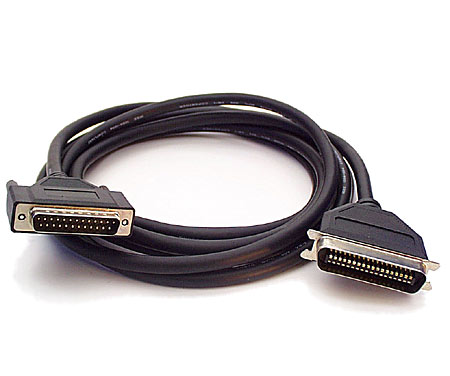
\includegraphics[scale=0.5]{./pics/IEEE1284Printercable_2007_04.jpg}
 \caption{IEEE 1284-Druckerkabel (Typ AB)} 	
\end{figure}
Der IEEE-Standard definiert die elektrischen Eigenschaften der Schnittstellen, die zu verwendenden Hardwareprotokolle und die zugehörigen Kabel. Für softwareseitige Protokolle wird auf Substandards verwiesen, die u.a. auch unabhängig von der eigentlichen Hardware agieren können. Heutzutage ist die parallele Schnittstelle (LPT) größtenteils durch modernere Schnittstellen, wie USB, ersetzt worden und erfährt nicht mehr die gleiche Bedeutung wie noch in den 1990er Jahren. 

 
\subsection{Aufgabenstellung und Projektziel}

Moderne PCs und Notebooks verzichten heutzutage bereits oft auf die parallele Schnittstelle und bieten für zusätzliche Peripheriegeräte dafür USB-Anschlüsse. Zwar sieht der ATX-Gehäusestandard noch farbliche Kennungen für LPT-Schnittstellen vor, bindend muss aber kein Hersteller diese Schnittstelle auf seinen Platinen integrieren. Um dennoch z.B. ältere Drucker in modernen Systemen verwenden zu können, bietet sich der Einsatz von PCI-Adapterkarten an, die über den PCI-Bus nach Außen hin einen Anschluss für die parallele Schnittstelle liefern. Die Implementierung eines Linux-Treibers einer solchen PCI-Adapterkarte soll Gegenstand dieser Projektarbeit sein. 

\subsection{Eingesetzte Hardware}  

Als Hardwareziel kommt eine PCI-Karte der Firma Exsys Inc (http://www.exsys.com) zum Einsatz, auf der ein Chip der Firma Moschip (http://www.moschip.com/) zum Einsatz kommt. Der dort verwendete Mikrocontroller stellt einen MCS9815-Chip dar, der die PCI zu LPT-Kommunikation übernimmt. Zwar findet sich im Linux-Kernel bereits ein Treiber für diesen Mikrokontroller, aufgrund geringer Projekteressourcen fehlt es jedoch an weiteren Alternativen. Da diese Projektarbeit eher dem lehrhaften Charakter einer studentischen Arbeit entspricht und die PCI-Karte den Projektteilnehmern bereits vorliegt, stellt die Entwicklung eines zusätzlichen Treibers für diese Karte nicht nur eine gute Übung dar, sondern ist auch gleichzeitig eine Herausforderung eine tatsächlich existierende Hardware unter dem Betriebssystem Linux zum Laufen zu bringen. Die Spezifikation dieses Mikrokontrollers hat die Firma Moschip offen gelegt, wodurch die Implementierung eines Treibers im Rahmen einer Projektarbeit ermöglicht wird.    


\section{Parallelportschnittstelle}

Die Parallelportschnittstelle ist wesentlich durch den IEEE 1284-Standard geprägt und definiert drei mögliche Steckertypen. Auf PC-Seite findet sich ein 25-poliger D-SUB.Stecker, der 1981 von IBM im PC eingeführt wurde (\textbf{Typ A}). Die 36-polige Centronics-Schnittstelle stellt den Stecker vom \textbf{Typ B} dar. Als Mini-Centronics werden Stecker vom \textbf{Typ C} bezeichnet, die ebenfalls über 36 Pole verfügen, aber deutlich kompakter daherkommen als übliche Centronics-Stecker (Abbildung \ref{fig:Alle IEEE 1284-Steckertypen im Vergleich}). 
\newpage
\begin{figure}[h!]
 \centering
 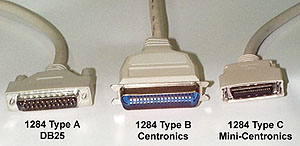
\includegraphics{./pics/ieee1284_types.jpg}
 \caption{Alle IEEE 1284-Steckertypen im Vergleich} 	
  \label{fig:Alle IEEE 1284-Steckertypen im Vergleich}
\end{figure}
\noindent
Üblicherweise wurden bei der häufig vorkommenden Verbindung zwischen PC und Drucker Kabel vom Typ AB eingesetzt. Dabei muss ein Mapping vom 25-poligen Typ A-Anschluss zum 36-poligen Typ-B-Anschluss vorgenommen werden (siehe Abbildung \ref{fig:Pinbelegung und -Verdrahtung bei üblichen Druckerkabeln}).  


\begin{figure}[h!]
 \centering
 
\includegraphics[scale=0.7]{./pics/ieee1284_pinbelegungAB.png}
 \caption{Pinbelegung und -Verdrahtung bei üblichen Druckerkabeln} 	
 \label{fig:Pinbelegung und -Verdrahtung bei üblichen Druckerkabeln}
\end{figure} 

\noindent
Die folgende Tabelle beschreibt die  Belegung und Bedeutung der einzeln Pins bei einem üblichen Druckerkabel. 
 \\ \\
 \begin{tabular}{|p{20mm}|p{20mm}|c|c|c|c|}
  \hline
	Pin (SUB-D-Type 25) & Pin (Centronics) & SPP Signal & Richtung Out & Register & Hardware\\ \hline
	1 & 	1	& 	Strobe				& 	Out		&	Control		&	Ja	\\ \hline
	2 & 	2	&	Data 0				&	Out		& 	Data		&     \\ \hline
	3 &	3	&	Data 1				&	Out		&	Data		&     \\ \hline
	4 &	4	&	Data 2				&	Out		&	Data		&     \\ \hline
	5 &	5	&	Data 3				&	Out		&	Data		&     \\ \hline
	6 &	6	&	Data 4				&	Out		&	Data		&     \\ \hline
	7 &	7	&	Data 5				&	Out		&	Data		&     \\ \hline
	8 &	8	&	Data 6				&	Out		&	Data		&     \\ \hline
	9 &	9	&	Data 7				&	Out		&	Data		&     \\ \hline
	10 & 	10	&	Ack				&	In		&	Status		&	    \\ \hline
	11 & 	11	&	Busy				&	In		&	Status		&	Ja  \\ \hline
	12 & 	12	&	Paper-Out/Paper-End		&	In		&	Status		&	    \\ \hline
	13 & 	13	&	Select				&	In		&	Status		&	    \\ \hline
	14 & 	14	&	Auto-Linefeed			&	Out		&	Control		&	Ja  \\ \hline
	15 & 	32	&	Error				&	In		&	Status		&	    \\ \hline
	16 & 	31	&	Reset				&	Out		&	Control		&	    \\ \hline
	17 & 	36	&	Select-Printer/Select-In	&	Out		&	Control		&	Ja  \\ \hline
	18 - 25	&	19-30	&	Ground	&	Gnd	&	&             \\ \hline
 \end{tabular}

\noindent \\
Um die einzelnen Pins mit Signalen zu belegen, sind drei Ports für die Behandlung der LPT-Schnittstelle im Rechner vorgesehen.  \\\\
 \begin{tabular}{|c|c|c|c|}
 \hline
\multicolumn{3}{|l|}{Portadresse}	&	Funktion\\  \hline 
278	&	378	&	3BC	&	Datenport \\  \hline 
279	&	379	&	3BD	&	Statusport \\  \hline 
27A	&	37A	&	3BE	&	Steuerport \\  \hline 
 \end{tabular} 
\noindent \\\\
In der Regel werden die Bereiche 278-27A und 378-37A verwendet. Der \textbf{Datenport} ist ein 8-Bit-Ausgagsport, der den Datenleitungen der parallelen Schnittstelle entspricht.  Der \textbf{Steuerport} setzt sich aus  Strobe, Auto-Feed, Reset, Select printer, IRC7 enable und Direction zusammen. 
\\ \\
 \begin{tabular}{|c|c|c|c|}
  \hline
Bit	&	Funktion	&	Pegel  \\ \hline
0	&	Strobe		&	0 \\ \hline
1	&	Auto-Feed	&	1\\ \hline
2	&	Reset		&	0\\ \hline
3	&	Select printer	&	1\\ \hline
4	&	IRQ7 enable	&	1\\ \hline
5	&	Direction	&	1\\ \hline
 \end{tabular} 
\noindent \\\\
Der \textbf{Statusport} ist ein 5 Bit-Port und setzt sich aus Error, Select Out, Paper Out, Acknowledge und Busy zusammen. \\

\noindent
\begin{tabular}{|c|c|c|c|}
  \hline
Bit	&	Funktion	&	Pegel\\ \hline
3	&	Fehler		&	0 	\\ \hline
4	&	Select out	&	1 \\ \hline
5	&	Paper out	&	1 \\ \hline
6	&	Acknowledge	&	0 \\ \hline
7	&	Busy		&	0 \\ \hline
 \end{tabular} 
\noindent \\\\
Unter Beachtung der ggf. auftretenden Invertierungen können diese Ports direkt beschrieben werden.\\\\

\subsection{Unterschiedliche Parallelporttypen und Modi}

Viele Hersteller verbesserten in der Vergangenheit die Centronics-Schnittstelle um eigene Betriebsmodi, aber erst durch die Standardisierung unter IEEE1284 wurden auch einheitliche Betriebsmodi vereinbart. Der IEEE-Standard sieht natürlich einen Modus zur Kommunikation mit Druckern vor, welcher als \textbf{SPP} (Standard Parallel Port)-Modus bezeichnet wird. Dieser Modus ist kompatibel zum alten Centronics-Standard. Zusätzlich sind in IEEE1284 auch bidirektionale, schnellere Betriebsmodi beschrieben, die als \textbf{EPP} (Enhanced Parallel Port) und \textbf{ECP} (Extended Capability Port) bezeichnet werden. Die folgende Übersicht geht auf die Besonderheiten der jeweiligen Betriebsmodi ein: \\\\

\noindent
\textbf{SPP: Standard Parallel Port}
\\
Der SPP-Modus ist IBMs Art und Weise aus dem Jahre 1981 den Paralallelport zu nutzen. Die Daten können jeweils nur unidirektional über die Datenleitungen gesendet werden. Mit dem SPP sind folgende Betriebsarten (nach IEEE1284) möglich:
\begin{itemize}
\item Compatible Mode:
      8-Bit-Parallelübertragung. Erlaubt den Betrieb von reinen Ausgabegeräten wie z.B. Druckern oder Plottern, die für Rückmeldeantworten die Signalleitungen nutzen können. 
\item Nibble Mode:
      Zur bidrektionalen Übertragung können hier die 5 Statusleitungen verwendet werden. Dabei werden vier Statusleitungen zur Dateneingabe genutzt. Daraus resultiert eine 4-Bit-Parallelübertragung (4 Bit = Nibble) von der Peripherie zum PC und eine 8-Bit-Parallelübertragung vom PC zur Peripherie.
\item Byte Mode:
      Bei späteren Ausführungen des SPP verwendeten einige Hersteller (wie IBM) acht bidrektionale Datenleitungen, wodurch eine 8 Bit Parallelübertragung ermöglicht wurde.\end{itemize}
\noindent
\textbf{EPP: Enhanced Parallel Port}
\\
EPP bei der parallelen Schnittstelle fand sich erstmals in Rechnern mit Intels 386SL-CPU. Durch EPP wird eine ``sehr schnelle'' parallele Schnittstelle bereitgestellt, die Datenraten von 500 KB/s bis zu 2MB/s ermöglicht, bleibt dennoch kompatibel zu alten SPP-Schnittstellen.
Die Leitungen der Schnittstelle sind jedoch anders spezifiziert als beim SPP.

\begin{itemize}
\item 4 Kontrolleitungen WRITE, DATA-STB, ADDR-STB, RESET (Ausgang)
\item 5 Statusleitungen INTR, WAIT, 3 x USER-DEF (Eingang)
\item 8 Adress-/Datenleitungen D0 - D7 (Ein+Aus) \end{itemize}
\noindent
\textbf{ECP: Extended Capability Port}
\\
ECP stellt eine Weiterentwicklung von EPP dar. Beim ECP-Modus werden die Daten lauflängenkodiert komprimiert vor dem Versenden. Die Kompression ist effizient in den Schnittstellenbausteinen der Hardware implementiert und besonders dann von Vorteil, wenn es gilt Bilddaten zu übertragen. Im Detail sieht ECP einen eigenen DMA-Kanal, eine FIFO-Pufferung für Hin- und Rückkanal und Datenkompression nach dem Runlenght-Encoding (RLE) Verfahren vor. Die Leitungen sind wie folgt spezifiziert:

\begin{itemize}
\item 4 Kontrolleitungen HOSTCLK, HOSTACK, 1284ACTIVE, REVERSEREQUEST (Ausgang)
\item Statusleitungen PERIPHCLK, PERIPHACK, ACKREV, XFLAG, PERIRQ (Eingang)
\item 8 Adress-/Datenleitungen D0 - D7 (Ein+Aus) \end{itemize}


\section{Der MosChip MCS9815 Controller}

Der MCS9815 ist ein Parallelport Controller Chip der Firma MosChip. Er kann
zwei Parallelports über das PCI Interface an das System anbinden und unterstützt alle
aktuellen Modi (SPP, PS2, EPP, ECP) der Parallelschnittstelle (vgl. Abbildung \ref{fig:blockdiagramm_mcs9815}).

\begin{figure}[h!]
 \centering
 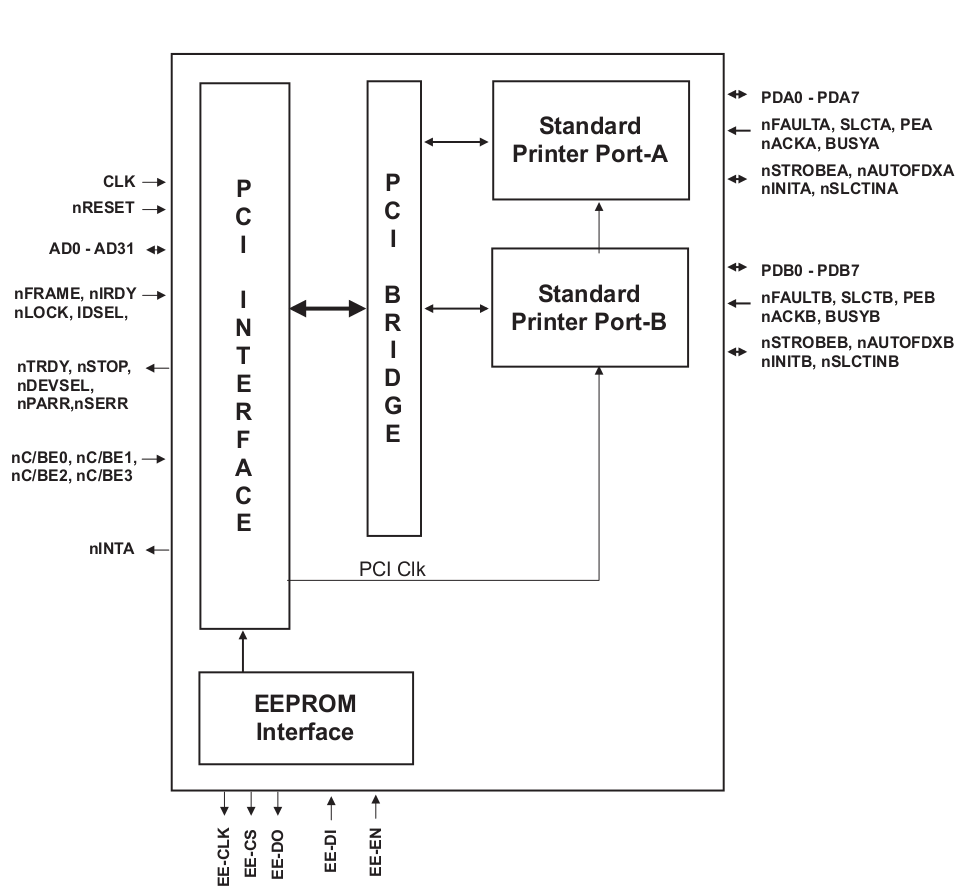
\includegraphics[bb=0 0 724 671,scale=0.5]{./pics/mcs9815_block_diagram.png}
 \caption{Blockdiagramm des MosChip MCS9815}
 \label{fig:blockdiagramm_mcs9815}
\end{figure}
\noindent
Einschränkungen des Chips ist die fehlende RLE-Kompression der Daten im ECP-Modus. Da dieser Modus aber
in der Praxis selten verwendet wird, ist diese Einschränkungen zu vernachlässigen.
Auch DMA (Direct-Memory-Access) unterstützt der Baustein nicht. Diese Informationen lassen sich dem Config-B Registers des
Chips entnehmen (oder auch dem Spezifikationsdokument des Chips \cite{net:3}).
Das aufwändige Handshaking beim EPP-Modus kann der MCS9815 in der Hardware abhandeln.

\section{Parport-Treiber in Linux}

\subsection{Aufbau des parport-Subsystems}


Da die Parallelportschnittstelle (umgangssprachlich) \textit{aus der Steinzeit} der PC-Entwicklung stammt, ist die Unterstützung
dafür im Linux-Kernel sehr gut. Das \verb|parport|-Subsystem ist für das Ansprechen von Geräten über die parallele Schnittstelle im Linux-Kernel verantwortlich.
Es besteht im Wesentlichen aus zwei Teilbereichen, einem abstrakteren Highlevel-System, das
die IEEE 1284-Kommunikation beherrscht und einem Lowlevel-System, was den Hardwarezugriff auf die einzelnen Ports
kontrolliert. Je nach Architektur und Plattform unterliegt dieses Lowlevel-System unterschiedlichen Implementierungen. Auf einem handelsüblichem IBM kompatiblen PC stellt das Modul \verb|parport_pc| den architekturspezifischen Teil bereit, das Modul \verb|parport| den generischen Teil (vgl. \cite{net:1} und Abbildung \ref{fig:parport_struktur}). 

\begin{figure}[h!]
 \centering
 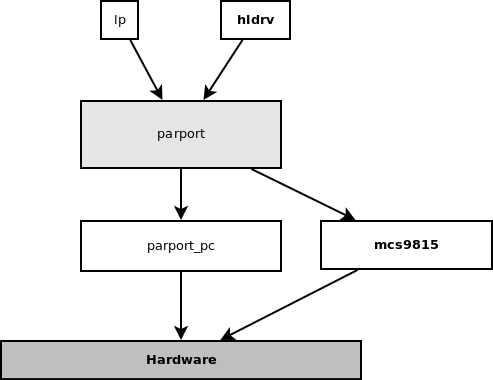
\includegraphics[scale=0.7,bb=0 0 493 380]{./pics/parport_struktur.png}
 \caption{Das parport-Modul stellt eine abstrakte Schnittstelle für Gerätetreiber bereit, die Brücke zur Hardware schlagen Architektur- und Hardware-
spezifische Treibermodule}
\label{fig:parport_struktur}
\end{figure}
\newpage
\noindent
Der hardwarespezifische Treiber registriert einen \emph{Port}\footnote{Port ist hier die logische Parallelschnittstelle, nicht zu verwechseln
mit dem I/O-Port (z.B. 0x378), der im PC für den Zugriff auf die Parallelporthardware verwendet werden kann} 
im \verb|parport| Subsystem. 
Dieses benachrichtigt alle registrierten Highlevel-Treiber (z.B. der Gerätetreiber \verb|lp| für Drucker) über den neuen Port. Der Lowlevel-Treiber stellt
Funktionen für den Zugriff auf Basisfunktionen des Ports bereit (vgl. \cite{net:1}).
\noindent
Eine teilaufgabe dieser Hausarbeit ist, einen Lowlevel-Treiber für einen speziellen Parallelport-Controller zu schreiben. Diese 
Funktionalität ist normalerweise im architekturspezifischen Modul \verb|parport_pc| integriert.

\subsection{Aufbau des MCS9815-Treibers}

In der Struktur des Treibersystems ordnet sich der im Rahmen dieser Arbeit zu erstellende Treiber als hardwarespezifischer Treiber
zwischen dem generischen parport-Modul und der eigentlichen Hardware ein. Er ist also der Adapter zwischen Hardware und parport-Modul 
(vgl. Abbildung \ref{parport_struktur}).

Die verwendete Schnittstellenkarte Exsys EX-41012 wird über den PCI-Bus an das System angebunden. Aufgabe des Treibers nach der generellen
Modulinitialisierung ist die Registrierung des Moduls als PCI-Treiber. Dies geschieht über den Aufruf der Kernelfunktion
\verb|pci_register_driver| mit einer entsprechenden \verb|pci_driver|-Struktur.

Sobald der Kernel die PCI-Karte mit der entsprechenden PCI-ID detektiert, wird die \verb|pci_probe| Funktion des Treibers aufgerufen, die
daraufhin mit der Initialisierung diverser Strukturen für das parport-Subsystem beginnt. Diese Aufgabe übernimmt die Funktion \verb|init_parport|
in der Datei\verb| mcs9815_main.c|.
Sie fragt den Kernel u.a. nach den I/O-Ports, über die die Kommunikation mit der Hardware abläuft. Der MCS9815-Controllerchip verwendet pro
Parallelport zwei Base-Address-Register (BAR). Wie die Parallelportregister auf die BARs der PCI-Hardware gemappt sind, zeigt 
Abbildung \ref{portkonf_mcs9815}.

\begin{figure}[h!]
 \centering
 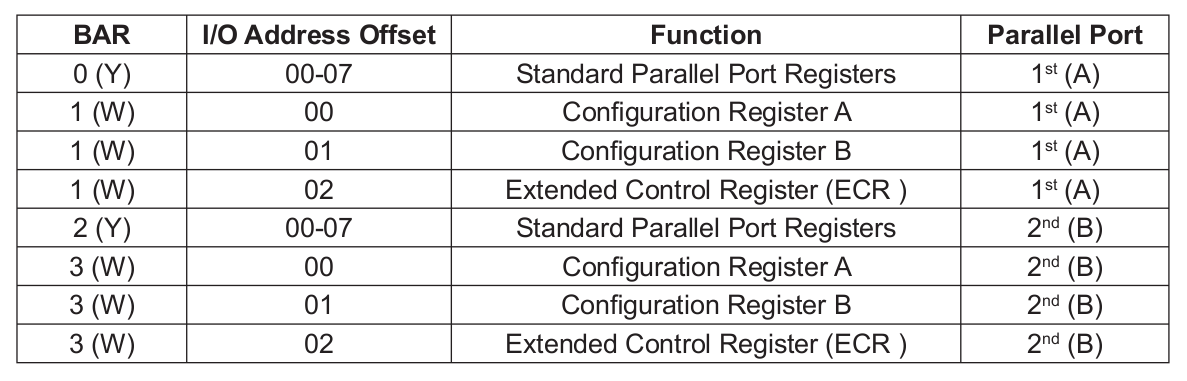
\includegraphics[scale=0.5]{./pics/mcs9815_ioports.png}
 \caption{Portkonfiguration des MosChip MCS9815}
 \label{portkonf_mcs9815}
\end{figure}

\newpage 
\noindent
Sobald die entsprechenden I/O-Ports bestimmt wurden, werden sie vom Treiber mit der Kernelfunktion \verb|request_region| allokiert.
Des weiteren füllt die \verb|init_parport| Funktion die Instanz der \verb|parport| Struktur mit sinnvollen Werten.
Die Struktur \verb|parport| repräsentiert eine logische Parallelschnittstelle.

\begin{verbatim}
struct parport {
    struct parport *next; /* next parport in list */
    const char *name;     /* port's name */
    unsigned int modes;   /* bitfield of hardware modes */
    struct parport_device_info probe_info;
                          /* IEEE1284 info */
    int number;           /* parport index */
    struct parport_operations *ops;
};\end{verbatim}
\noindent
Die Struktur enthält auch einen Verweis auf die wichtige Struktur \verb|parport_operations|.
Wie auch die Struktur \verb|file_operations| bei einem Dateisystemtreiber enthält die 
Struktur \verb|parport_operations| u.a. Funktionszeiger auf die vom Treiber unterstützten
Parallelportfunktionen.

\begin{verbatim}
struct parport_operations {
    /* IBM PC-style virtual registers. */
    void (*write_data)(struct parport *, unsigned char);
    unsigned char (*read_data)(struct parport *);

    void (*write_control)(struct parport *, unsigned char);
    unsigned char (*read_control)(struct parport *);
    unsigned char (*frob_control)(struct parport *, unsigned char mask, unsigned char val);

    unsigned char (*read_status)(struct parport *);

    /* IRQs. */
    void (*enable_irq)(struct parport *);
    void (*disable_irq)(struct parport *);

    /* Data direction. */
    void (*data_forward) (struct parport *);
    void (*data_reverse) (struct parport *);

    /* For core parport code. */
    void (*init_state)(struct pardevice *, struct parport_state *);
    void (*save_state)(struct parport *, struct parport_state *);
    void (*restore_state)(struct parport *, struct parport_state *);

    /* [..] */

    size_t (*compat_write_data) (struct parport *port, const void *buf, size_t len, int flags);
    size_t (*nibble_read_data) (struct parport *port, void *buf, size_t len, int flags);
    size_t (*byte_read_data) (struct parport *port, void *buf, size_t len, int flags);
    struct module *owner;
};\end{verbatim}
\noindent
Das generische parport Modul des Kernels verwendet diese Funktionszeiger um über das hardwarespezifische Modul mit 
der tatsächlichen Hardware zu kommunizieren. Das Parport-Modul muss für den Betrieb geladen sein.
Die Implementierung dieser Funktionen befinden sich in der Datei \verb|mcs9815_ops.c|. 

Mit den entsprechend initialisierten Strukturen registriert der Treiber mit dem Aufruf der Funktion \verb|parport_register_port| einen Parallelport im Kernel.
Um diesen Parallelport den Gerätetreibern im System bekannt zu machen, muss die Funktion \verb|parport_announce_port| aufgerufen werden.
Wie ein (highlevel) Gerätetreiber das parport-Subsystem verwendet wird im folgenden Abschnitt erläutert.
Nach dem Bekanntmachen des Treibers ist die Initialisierung abgeschlossen und der Treiber kann verwendet werden.
Beim Entfernen des Treibers aus dem System wird der Parallelport vom Kernel abgemeldet, die Strukturen abgemeldet und schließlich das PCI-Gerät 
abgeschaltet.

\subsection{Highlevel Testtreiber}

Nach dem Vorbild des \verb|lp|-Treibers unter Linux, welcher einen Highevel-Lineprinter für die parallele Schnittstelle darstellt, wurde ein Testtreiber entwickelt. Als Testgerät wurde an den LPT-Anschluss der PCI-Karte eine mit LEDs ausgestattete Platine angeschlossen, die durch jeweiliges An- und Ausschalten der einzelnen Lichter den Zustand des Datenregisters der parallelen Schnittstelle anzeigt. Das Ziel der Entwicklung war es nun einen Treiber zu entwickeln, der den Datenport regelmäßig mit Inhalt befüllt, welcher dann durch die LEDs der Platine entsprechend visualisiert dargestellt wird. Auf der LED-Platine wird dann entsprechend zum Zahlenwert binär hochgezählt. Erreicht der Zählerstand einen Wert größer als 255, wird auf der Platine von Neuem angefangen zu zählen.
Ein solch wechselnder Inhalt wird über einen einfachen Zähler realisiert, der in einem geiwssen Zeitintervall den Zählerstand um eins inkrementiert. Der Linuxkernel bietet hierfür Timer-Funktionalität an, die durch das Einbinden von \verb|<linux/timer.h>| genutzt werden können. Durch \verb|init_timer(&timer)| wird der Timer initialisiert. Die Methode erwartet eine Referenz auf ein Struct vom Typ timer\_list. 
\begin{verbatim}
  static struct timer_list timer;
  static int timer_interval = 500;
  // Initialize timer
  init_timer(&timer);
  timer.expires = jiffies + timer_interval;
  timer.data = 0;
  timer.function = timer_strobe;
  add_timer(&timer);
\end{verbatim}
\noindent
Nach der Timerinitialisierung werden zusätzliche Parameter festgelegt. Insbesondere ist der Funktionspointer auf die Methode von Bedeutung, die immer dann ausgeführt werden soll, wenn der festgelegte Zeitinterval von 500ms abgelaufen ist. In diesem Fall wird die methode \verb|timer_strobe| jeweils aufgerufen.
\noindent \\
Der Testtreiber verwendet das \verb|parport|-Subsystem und registriert sich an diesem als Treiber. Über vorhandene Methoden zum Schreiben auf den Parallelport und weitere Funktionalität wird die Kommunikation mit dem Parport-Subsystem realisiert. Um zunächst den Treiber am Subsystem zu registrieren, wird ein Struct vom Typ \verb|parport_driver| benötigt.
\newpage
\begin{verbatim}
#include <parport.h>

struct parport_driver {
  const char *name;
  void (*attach) (struct parport *);
  void (*detach) (struct parport *);
  struct parport_driver *next;
};
\end{verbatim}
\noindent
In diesem Struct werden der Name des Treibers, sowie Funktionenszeiger auf Methoden festgelegt, um die Abläufe zu steuern, die beim Aufsetzen/Entfernen des Treibers von Bedeutung sind. Mit den Informationen aus diesem Struct kann das Device beim Parport-Subsystem registriert werden durch bereitgestellte Methode:
\begin{verbatim}
int parport_register_driver(struct parport_driver *driver);
\end{verbatim}

\noindent Nach dem Registrieren des Treibers am Parport-Subsystem wird vom Kernel zu gegebener Zeit die Attach-Methode vom \verb|parport_driver| Struct aufgerufen. In der Attach-Methode wird dann das zu verwendende Gerät ermittelt. Ein Struct vom Typ \verb|pardevice| wird dann von der folgenden Methode zurückgegeben:

\begin{verbatim}
#include <parport.h>

struct pardevice *parport_register_device(struct parport *port, 
  const char *name, 
  int (*pf) (void *), 
  void (*kf) (void *), 
  void (*irq_func) (int, void *, 
  struct pt_regs *), 
  int flags, void *handle);
\end{verbatim}
\noindent
Um den konkreten Betriebsmodus der parallelen Schnittstelle auszuhandeln, wird die Methode \verb|parport_negotiate| verwendet.

\begin{verbatim}
#include <parport.h>
int parport_negotiate(struct parport *port, int mode);
\end{verbatim}
\noindent
In diesem Fall könnte z.B. über die Konstante \verb|IEEE1284_MODE_COMPAT| der Kompatibilitätsmodus (SPP) eingestellt werden. 
\noindent \\\\
In der \verb|timer_strobe|-Methode wird jeweils auf den Parallelport geschrieben. Hierfür ist eigentlich die entsprechende Write-Methode vorgesehen:

\begin{verbatim}
#include <parport.h>

ssize_t parport_write(struct parport *port, const void *buf, size_t len);
\end{verbatim}
\noindent
Beim Testen des entworfenen Treibers trat bei der Verwendung dieser Methode jedoch ein Problem auf. Unter Verwendung des normalen \verb|parport_pc|-Moduls als low-level-Treiber kam es beim Aufruf der write-Methode zu einem Systemabsturz. Interessanterweise konnte dieses Problem bei der Verwendung des eigenen low-level-Treibers nicht reproduziert werden. Mit dem (in dieser Projektarbeit entstandenden) mcs9815-Modul als Ersatz für das parport\_pc-Modul funktionierte der Aufruf der Write-Methode fehlerfrei. Damit aber auch das standard parport\_pc-Modul des Linux-Kernels mit dem High-Level-Treiber funktioniert, wurde ein anderer Schreibaufruf vewendet. Über die Parport-Operations des Device-Structs wird eine zusätzliche write-Methode zur Verfügung gestellt, die mit beiden Modulen funktioniert. Die entsprechende Passage ist im Code wie folgt hinterlegt

\begin{verbatim}
// Writes the countvalue into our port
  dev->port->ops->write_data(dev->port, countvalue);
// Alternative:
// written = parport_write(dev->port, &countvalue, 1);
// dev->port->ops->write_data is  probably faster as parport_write 
// has an additional call to compat_write_data() in between. 
// Additionally parport_write() only works with our mcs9815 
// driver and freezes with the default parport_pc driver...
\end{verbatim}
\noindent
Beim Entladen des Highlevel-Treiber-Moduls wird die \verb|parport_unregister_device| noch angewendet.

\begin{verbatim}
void parport_unregister_device(struct pardevice *dev);
\end{verbatim}

\section{Fazit}

Hauptaugenmerk dieser Arbeit war die die Entwicklung eines Treibers für den MCS9815-Chipsatz unter Berücksichtigung des Parport-Subsystems. Der Chipsatz befindet sich auf einer PCI-Karte, so dass über den PCI-Bus die Möglichkeit bereitgestellt wird eine (zusätzliche) Parallelportschnittstelle dem System zur Verfügung zu stellen. Mit den erlernten Kenntnissen aus der Vorlesung und dem Praktikum konnte die Aufgabe aus sicht der Beteiligten dieser Arbeit gut umgesetzt werden, war aber dennoch stets fordernd. Es konnte ein guter Einblick in den Ablauf bei der Entwicklung eines richtigen Linux-Treibers gewonnen werden. Eine Erkenntnis dieser Arbeit ist sicherlich, dass klar wurde wie viel Herzblut und Arbeit die Linux-Treiberentwickler in das freie Betriebssystem stecken, um möglichst viel Hardware ansprechen zu können. Dadurch, dass die Spezifikation des Chipsatzes offenlag konnte aus Projektsicht die Arbeit so durchgeführt werden, wie auch tatsächliche Kernel-Treiberentwickler die Aufgabe gelöst hätten. Die Aufgabenstellung beim Entwickeln eines Treibers verfolgt also ein klares Muster. Zunächst muss man sich mit der Hardware auseinandersetzen, die man ansprechen möchte. Schnittstellenbeschreibungen und Spezifikationen sind hier vön Nöten. Für die geleistete Arbeit mussten Kenntnisse über den verwendeten Chipsatz und über die Verwendung des PCI-Bus und der parallelen Schnittstelle unter Linux gesammelt werden. Es überrascht, dass das sehr alte Parport-Subsystem unter Linux auch heute noch recht elegant von der Architekturseite her erscheint. Durch die Abstraktion zwischen Highlevel- und Lowlevel-Treibern, können Entwickler eine klare Trennung von der eigentlichen Gerätelogik und dem Ansprechen benötigter Ports vornehmen. Das Parport-Subsystem hilft dem Highlevel-Treiberentwickler dabei das eigene Gerät am System zu registrieren und es zu verwenden. Erst der Lowlevel-Treiber geht tatsächlich auf die Bitebene herunter und beschreibt entsprechende Ports. Das Parport-Subsystem delegiert dabei zwischen beiden Welten. Wenn klar ist, wie die Hardware anzusprechen ist, können sich Entwickler an die Entwicklung des eigenen Treibers machen und ggf. von entsprechenden Abstraktionsschichten, wie dem Parport-Subsystem, profitieren. Zum Status des entwickelten Treibers ist zu sagen, dass er nur im SPP-Modus getestet werden konnte. Die EPP-Funktionen sind zwar vollständig implementiert, aber mangels eines geeigneten Testgerätes konnte leider die Funktionalität nicht erschöpfend geprüft werden. Die ECP-Funktionen konnten nicht vollständig implementiert und getestet werden, da das Einbauen dieser zusätzlichen Funktionalität den Zeitrahmen der Arbeit zusätzlich gesprengt hätte. Die getätigte Projektarbeit hat jedoch idealerweise viele Bereiche der Vorlesung abgedeckt, in dem z.B. die Kommunikation mit dem PCI-Bus, Timer-Funktionalität oder die parallele Schnittstelle verwendet werden konnte. Die Projektarbeit rundet also die Inhalte und gewonnenen Erkenntnisse der Vorlesung in einer schönen Art und Weise ab. 


\newpage
\cleardoublepage
\nocite{*}
%{\footnotesize\singlespacing{{\bibliographystyle{jurabib}
%{\footnotesize\singlespacing{{\bibliographystyle{jureco}
%{\footnotesize\singlespacing{{\bibliographystyle{apacite}
\bibliography{literatur}


\end{document}